\textbf{Цель работы:} \\\indent
1) измерение частоты колебаний и длины волны при резонансе 
зуковых колебаний в газе, заполняющем трубу;\\\indent
2) определение показателя адиабаты с помощью уравнения состояния
идеального газа.\\ \indent
\textbf{Оборудование:} звуковой генератор, электронный осциллограф, 
микрофон, телефон, раздвижная труба, теплоизолированная турба, 
баллон со сжатым углекислым газом, газгольдер.\\ 

\section*{Теоретические сведения}

Скорость звука в газах поределяется как:
\begin{equation}
    c = \sqrt{\gamma \frac{R T}{\mu}}
\end{equation}

Если длина трубы $L$ равна целому числу полуволн ($L = n\frac{\lambda}{2}$),
волна, отраженная от торца трубы совпадает по фазе с падающей. Поэтому 
они усиливают друг друга и возникает резонанс. Скорость звука при 
этом связана с длиной волны как: 
\begin{equation}
   c = \lambda f
\end{equation}
\indent
Рассмотрим 2 способа образования резонансая:\\\indent
1)При $f = const$, изменяя длину трубы.\\\indent
2)При $L = const$, изменяя частоту звуковых колебаний. Тогда
\begin{align}
    L &= \frac{\lambda_1}{2} n = \frac{\lambda_2}{2} (n+1)\dots = \frac{\lambda_{\text{k+1}}}{2}(n + k)\\
    f_1 &= \frac{c}{\lambda_1} = \frac{c}{2L} n\\
    f_2 = \frac{c}{2L}(n + 1) &= f_1 + \frac{c}{2L} k \Rightarrow f_{\text{k+1}} = f_1 + \frac{c}{2L} k
\end{align}

\section*{Экспериментальная установка}
Звуковые колебания возбуждаются телефоном Т и улавливаются микрофоном М. 
Возникающий в нем сигнал отображается на осциллографе ЭО. 

\begin{figure}
    \centering
    \begin{subfigure}{0.45\linewidth}
        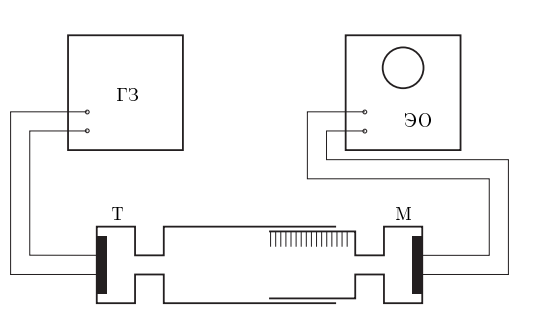
\includegraphics[width=9cm]{setup1.png}
        \caption{Установка для измерения скорости звука при подвижной трубе}
    \end{subfigure}
\hfill
    \begin{subfigure}{0.45\linewidth}
        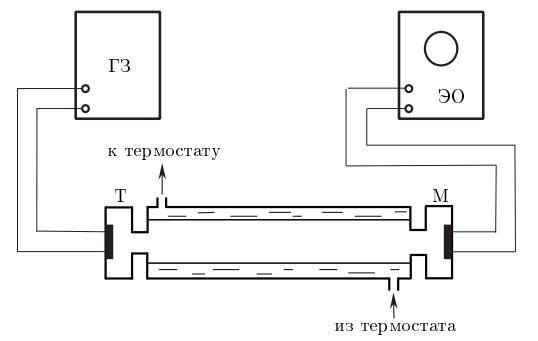
\includegraphics[width=9cm]{setup2.png}
        \caption{Установка для изучения зависимости скорости звука от температуры}
    \end{subfigure}
\end{figure}



